\chapter{Analyse}

\section{Recherche}
\label{sec:recherche}

\subsubsection{Bezeichnung}
Der Ausdruck \gls{glos:droneLabel} kommt vom niederdeutschen Wort \textit{"`drone"'}, welches wiederum seinen Ursprung beim indogermanischen Wort \textit{"`dhren"'} findet. Die Bedeutung dieses Wortes lautet "`brummen"' oder "`dröhnen"'. \footcite{Geschichte_der_Drohne_-_Nachrichten_Print_-_DIE_WELT_-_Wissen_Print_DW_-_DIE_WELT_2015-03-21}

\begin{framed}
	\textit{Definition: }\textbf{\gls{glos:droneLabel}}\\
	Als \gls{glos:droneLabel} wird ein unbemanntes Luftfahrzeug bezeichnet. Die Steuerung kann entweder manuell oder autonom erfolgen.\\
	Quelle:
	\fullcite{Drone_Define_Drone_at_Dictionary.com_2015-03-21}
\end{framed}

\subsection{Geschichte der Drohne}

\subsubsection{Frühe Entwicklung}
Eine der allerersten bekannten \gls{glos:droneLabel} war wohl von den Brüder Mongolfier (1783) aus Frankreich, ein unbemannter Heissluftballon. \footcite{Kleine_Geschichte_der_Drohnen_-_Nachrichten_Print_-_WELT_KOMPAKT_-_Lifestyle_-_DIE_WELT_2015-03-21}
\footcite{Unbemannte_Luftfahrt__Wikipedia_2015-03-22}

\subsubsection{Waffenträger}
Später wurde das Potenzial von \glspl{glos:droneLabel} besonders für kriegerische Zwecke erforscht und entwickelt.

\begin{wrapfigure}{R}{0.4\textwidth}
	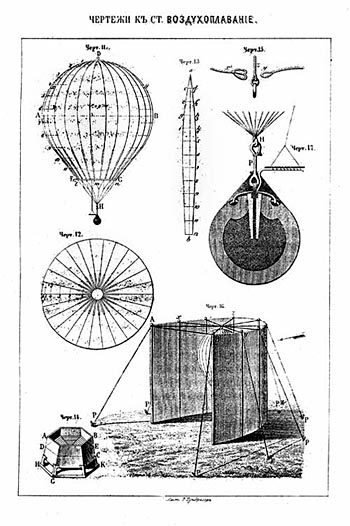
\includegraphics[width=1.0\linewidth]{images/analysis/balloonbombs1849.jpg}
 	\caption[Bombing by Balloon, 1848]{Bombing by Balloon, 1848 (Quelle: \fullcite{Remote_Piloted_Aerial_Vehicles_2015-03-21})}
\end{wrapfigure}
So wurden bereits 1849, vom österreichischen Königsreich, unbemannte Heissluftballone mit Bomben im Krieg gegen Venedig losgeschickt.
Weder die "`\gls{glos:droneLabel}"' selbst, noch das Abwerfen der Bombe konnte aktiv gesteuert werden.
Die Heissluftballone flogen mit dem Wind und die Bomben wurde per Zeitzünder gezündet. Tatsächlich erreichten einzelne Ballone ihr Ziel und konnten Schaden anrichten, andere jedoch wurden vom Wind zurück geweht und zerstörten das eigene Territorium Österreichs. \footcite{Remote_Piloted_Aerial_Vehicles_2015-03-21}

Während dem \textit{Ersten Weltkrieg} wurden die ersten unbemannten Flugzeuge von den Amerikanern entwickelt.
Mit diesen wurden vordefinierte Routen abgeflogen und es konnten \textit{Flugtorpedos} abgeworfen werden, welche wie die Flugzeuge selbst, mit Hilfe von gyroskopischen Stabilisierer und Aneroidbarometer zwar Richtung und Höhe halten konnten, jedoch nicht per Funk steuerbar waren.

Die ersten funkgesteuerten \glspl{glos:droneLabel} wurde erst nach dem Krieg 1918 fertig.
Nebst den Amerikanern, hatten auch die Briten 1925 ihren ersten Drohnenflug durchgeführt. Diese konnte etwa 300\,Meilen (ca. 483\,km) mit einer Geschwindigkeit von 190\,mph (ca. 306\,km/h) zurücklegen.\footcite{Informatik_und_Gesellschaft_2015-03-21}

Da der Krieg vorbei war, wurden die \glspl{glos:droneLabel} hauptsächlich für Jagd-Trainings der Armee genutzt.

Mit den Jahren wurden die \glspl{glos:droneLabel} immer weiter verbessert und werden heute aktiv gegen terroristische Aktivitäten verwendet.

\subsubsection{Weitere Zwecke}
% http://diepresse.com/home/politik/innenpolitik/1385181/Die-Geschichte-der-Drohnen
Nebst den erwähnten Waffenträger gibt es auch diverse weitere Aufgaben für \glspl{glos:droneLabel}: Beobachtungen (z.B. Aufklärungen, Luftaufnahmen, Wetterbeobachtungen, Filmproduktionen), Messungen an Orten die für Menschen ungeeignet oder schädlich sind oder Transporte.

Obschon viele Aufgabenbereiche gewaltfrei sind, dienen \glspl{glos:droneLabel} trotzdem mehrheitlich polizeilichen oder militärischen Organisationen.\footcite{Die_Geschichte_der_Drohnen_DiePresse.com_2015-03-21}

\subsubsection{Heutige Einsätze von Drohnen}
Seit 2013 werden, in Grand Forks County im US-Bundesstaat North Dakota, \glspl{glos:droneLabel} zur Verbrecherjagd eingesetzt, resp. zur Personensuche.\footcite{Grand_Forks_Drone_Assisted_Policing_2015-08-28}
Zudem darf in Grand Forks County seit August 2015 eine Drohnen sogar mit einem Taser bestückt werden. \footcite{First_State_Legalizes_Taser_Drones_for_Cops_Thanks_to_a_Lobbyist_The_Daily_Beast_2015-08-28}

Auch Amazon kündet ihren "`\textit{Prime Air}"'-Service an, der Pakete direkt vor die Haustür liefert.\footcite{Amazon_Prime_Air_2015-08-28}

Im Jahr 2014 wurde der Einsatz für landwirtschaftliche Zwecke erprobt und auch die \gls{glos:dhlLabel} führte Testlieferungen mit \glspl{glos:droneLabel} aus. \footcite{Kleine_Geschichte_der_Drohnen_-_Nachrichten_Print_-_WELT_KOMPAKT_-_Lifestyle_-_DIE_WELT_2015-03-21}


\section{Quadrocopter Steuerung}
\begin{wrapfigure}{R}{0.4\textwidth}
	\vspace{-3\baselineskip}
	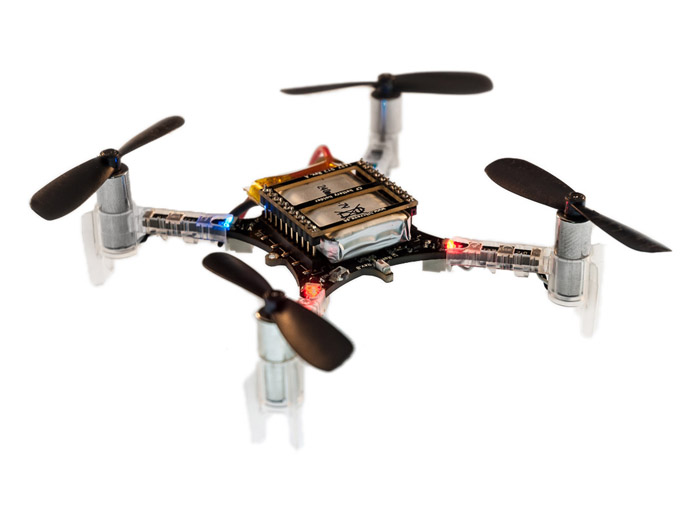
\includegraphics[width=1.0\linewidth]{images/analysis/crazyflize.jpg}
	\caption[Crazyflie 2.0]{Crazyflie 2.0 (Quelle: \fullcite{Crazyflie_2.0_Seeedstudio_2015-03-22})}
	\vspace{-1.5\baselineskip}
\end{wrapfigure}
Der Quadrocopter eignet sich als \gls{glos:droneLabel}, da die Steuerung ausschliesslich über die vier Rotoren realisiert wird.
Weitere mechanische Steuerkomponente entfallen, was die Komplexität des Luftfahrzeuges deutlich vereinfacht.
Je zwei der Rotoren drehen in dieselbe Richtung (im bzw. gegen den Uhrzeigersinn) und stehen sich gegenüber.

Generell gilt für vorliegendes Dokument, insofern nicht anders vermerkt oder aus dem Kontext ersichtlich, dass der Begriff Drohne mit dem Begriff Quadrocopter gleichzustellen ist (davon ausgeschlossen ist \secref{sec:recherche}).


\subsection{Steuerung}
Bezüglich der Flugeigenschaften entspricht ein Quadrocopter am ehesten einem Hubschrauber und gehört ebenfalls zur Kategorie der  \gls{glos:vtolLabel}-Flugzeugen.
Es sind jegliche Steuermöglichkeiten im dreidimensionalen Raum möglich (steigen/sinken "`\textit{thrust}"', gieren/drehen "`\textit{yaw}"', nicken "`\textit{pitch}"' und rollen "`\textit{roll}"').

Durch das, dass die Rotoren in entgegengesetzte Richtungen drehen, hebt sich das auf das Traggestell übertragene Drehmoment auf und der Quadrocopter kann ohne Drehung fliegen.
Um sich nun in eine Richtung zu \textit{gieren}, werden die Drehzahlen von jeweils zwei gegenüberliegende Rotoren gleichmässig verändert, so dass der Drehmoment auf das Traggestell nicht mehr neutralisiert wird und sich so eine Drehung ergibt.

Um dem Piloten die Steuerung zu erleichtern, befinden sich oft verschiedenfarbige Markierungen oder LED's an der Vorder- oder Rückseite des Quadrocopters.
Die Steuerung erfolgt üblicherweise aus relativer Sicht der Drohne und erfordert somit ein Umdenken des Piloten.\footcite{Quadrocopter__Wikipedia_2015-03-22}

\newpage
\subsection{Bereits bestehende Arbeiten}
Da Drohnen erst während der letzten Zeit aufgekommen und erschwinglich geworden sind, lassen sich sehr viele Drohnen-Projekte mit verschiedenster Hardware finden.
Folgend wird der Fokus besonders auf Projekte mit einer Gestensteuerung und deren Steuerungsmöglichkeiten gelegt.


\subsubsection{Drohnen}
Für viele der gefundenen Projekte wurden, nebst der Crazyflie, die \textit{AR.drone} von Parrot verwendet.\footcite{AR_Drone_2.0_Parrot_2015-04-29}
Die AR.drone ist erheblich grösser als die Crazyflie, was zur Flug-Stabilität beiträgt.
Mit an Board ist eine Kamera.
Obwohl die AR.drone einige Vorteile mit sich bringt und die Kosten nur wenig höher sind als bei der Crazyflie, hat Parrot eine deutlich kleinere Community und eine weniger ausführliche Entwicklerdokumentation.
Die Crazyflie richtet sich hauptsächlich an Entwickler, während die AR.drone auch normale Nutzer anspricht.
Aufgrund der grösseren Community und der ausführlicheren Entwicklerdokumentation wurde für diese Arbeit die Crazyflie verwendet.

\subsubsection{Steuermöglichkeiten}
Zusammengefasst können die Steuerungsmöglichkeiten in folgende Kategorien eingeteilt werden:
\begin{itemize}

	\item \textbf{Steuerung mit offener Hand:}
	Eine solche Steuerung basiert auf der Erkennung der offenen Hand.
	Meist befindet sich der Sensor für die Gestenerkennung unterhalb der Hand und kann so stabil aufgestellt werden.

		\begin{itemize}

			\item \textbf{Handrichtungs-basierte Steuerung:}
			Diese Steuerung ist an der Benutzung eines gewohnten Hebels oder Joysticks angelehnt. Die Drohne bewegt sich analog der Hand. Dabei spielt der Winkel der Hand keine Rolle.
			Beispielsweise bedeutet eine Hand die vor dem Zentrum des Sensores liegt, dass die Drohne nach vorne fliegen soll. Das Pitch-Manöver wird oft durch spezielle Gesten wie \textit{Kreisen} umgesetzt.
			Ein Beispiel wird im Blog von Leap Motion vorgestellt.\footcite{The_Beginning_of_a_Drone_Revolution_Leap_Motion_Blog_2015-04-29}

			\item \textbf{Handpositions-basierte Steuerung:}
			Bei der handpositions-basierten Steuerung, stellt die Position der Hand, effektiv die Position der Drohne dar. Der Winkel der Handhaltung, soll des Winkels der Drohne entsprechen.
			Wo genau sich die Hand über dem Sensor befindet, ist ausser für den Thrust, nicht relevant.
			Eine erfolgte Umsetzung ist auf Youtube vorhanden.\footcite{Flying_the_Crazyflie_with_Leap_Motion_YouTube_2015-04-29}
		\end{itemize}

	\item \textbf{Lenkdrachen-Steuerung:}
	Bei dieser Steuerung erfolgen die Kommandos ähnlich wie bei einem Lenkdrachen.
	Am Besten stellt man sich zwei unsichtbare Eisenstangen vor, die seitlich an der Drohne befestigt sind und von dort zu den Händen führen. Durch bewegen der imaginären Stangen kann die Drohne in verschiedene Positionen bewegt werden.
	Um diese Gesten zu erkenne, wird der Sensor oder die Kamera meist frontal, z.B. am Bildschirmrand, befestigt.
	Bei einer Implementation am \textit{Hackathon} in München, wird als Startzeichen das Heben der Daumen verwendet.\footcite{Drones_Fly_Hands_Free_with_Gestural_Technology_2015-04-29}

	\item \textbf{Steuerung mit \glspl{glos:wearableLabel}:}
	Anstatt Gesten wirklich zu erkennen, kann eine Steuerung auch durch ein \gls{glos:wearableLabel} am Handgelenk oder in der Hand erfolgen.
	Da aktuell den \glspl{glos:wearableLabel} eine grosse Aufmerksamkeit der Medien geschenkt wird, ist in absehbarer Zeit eine starke Entwicklung von \glspl{glos:wearableLabel} zu erwarten (z.B. das Myo Armband\footcite{Myo_Gesture_Control_Armband_-_Wearable_Technology_by_Thalmic_Labs_2015-08-28}).
	Momentan sind \glspl{glos:wearableLabel} den Gestenerkennungssensoren noch unterlegen.
	Trotzdem wird auf Hackday eine Drohne mit einer \gls{glos:wearableLabel}-Steuerung vorgestellt.\footcite{Wearable_Gesture_Controlled_Drone_Hackaday_2015-04-29}
\end{itemize}

Da die handpositions-basierte Steuerung der intuitivsten und einfachsten Steuerung entspricht, und es bisher nur wenige dokumentierte  Implementationen gibt, wird in vorliegender Arbeit diese implementiert.
Im Gegensatz zur soeben erwähnten, bereits existierenden handpositions-basierte Steuerung, soll die zu implementierende Steuerung jegliche Steuermanöver (Yaw, Pitch, Roll, Thrust) unterstützen.
Zudem soll die Steuer-Initialisierung und die Steuerung sicher ablaufen. Dazu werden verschiedene Zustände implementiert, in der sich die Steuerung befinden kann.

Es wird der Gestensensor von Leap Motion verwendet (weitere Informationen zum Sensor sind im \secref{subsec:leapmotion} beschrieben).


%\subsubsection{Sensoren Integration auf bestehende Steuerungen}

\clearpage % because floating doesn't work correctly
\section{Ist-Analyse}

%\subsection{System}
In der Ausgangslage gibt es zwei Fremdsysteme (blau eingefärbt): der Leap Motion (\secref{subsec:leapmotion}) und die Crazyflie (\secref{subsec:isAnalyseDrone}).

%\vspace{-1\baselineskip}
\begin{figure}[H]
	\centering
	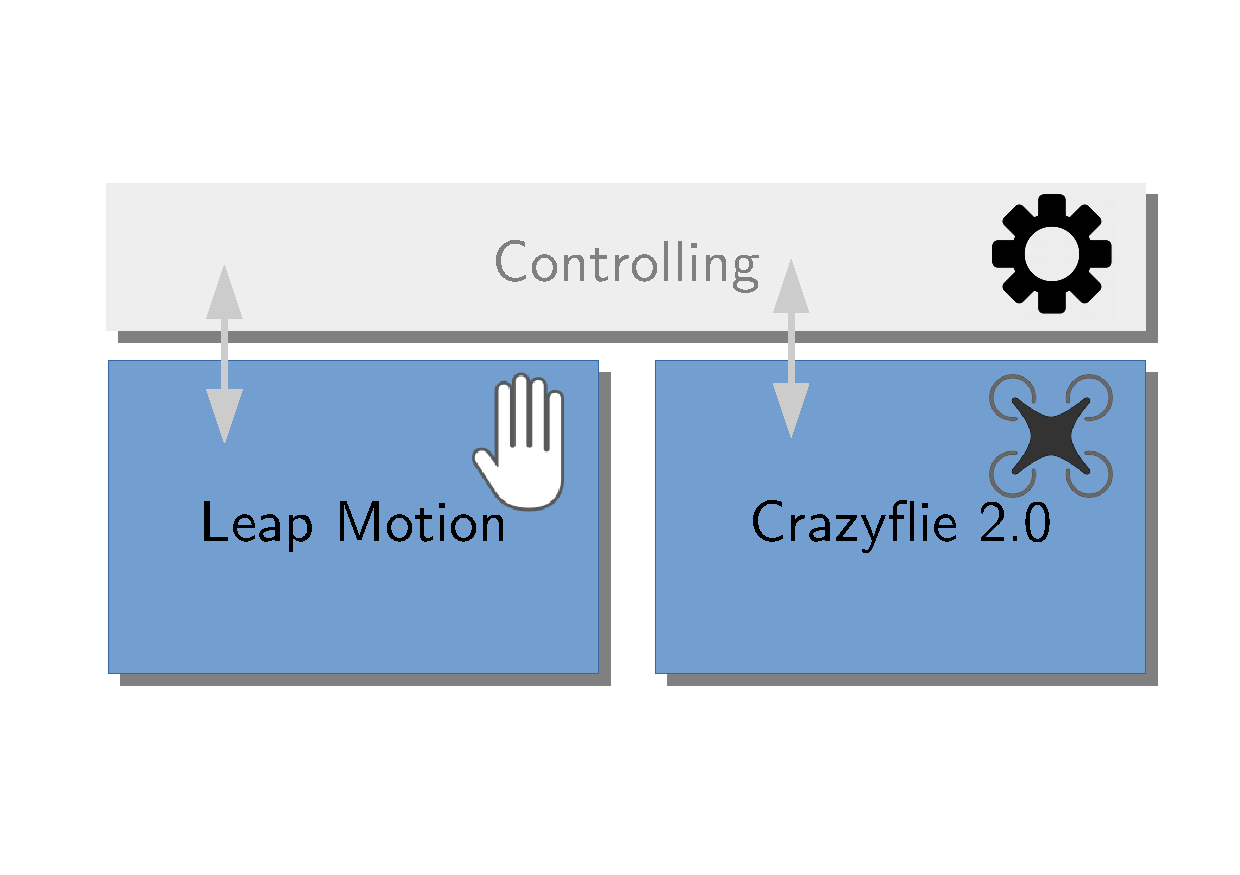
\includegraphics[width=0.8\textwidth]{figures/system_is.pdf}
	\caption{System-Überblick: Ist-Zustand}
	\vspace{-3\baselineskip}
\end{figure}

Beide Systeme sind Open Source, haben eine aktive Community und funktionieren selbstständig und vollständig.
Dazu soll eine Steuerung (Controlling) umgesetzt werden, welche die zwei Systeme verbindet, so dass die Drohne via Gesten gesteuert werden kann.

Folgend werden die zwei Systeme genauer beschrieben.

\newpage
\subsection{Gestensensor}
\label{subsec:leapmotion}
\begin{wrapfigure}{R}{0.4\textwidth}
	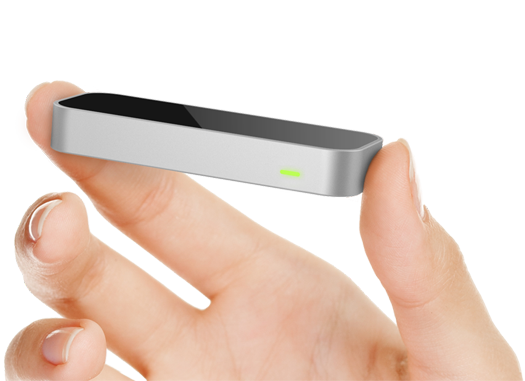
\includegraphics[width=1.0\linewidth]{images/analysis/leap_simple.png}
	\caption[Leap Motion Sensor]{Leap Motion Sensor (Quelle: \fullcite{Move_Over_Kinect:_Early_Gestural_Musical_Demos_for_Leap_Motion_Look_Terrific_-_Create_Digital_Music_2015-03-27})}
\end{wrapfigure}
%too much: not used
%\begin{wrapfigure}{l}{0.4\textwidth}
%	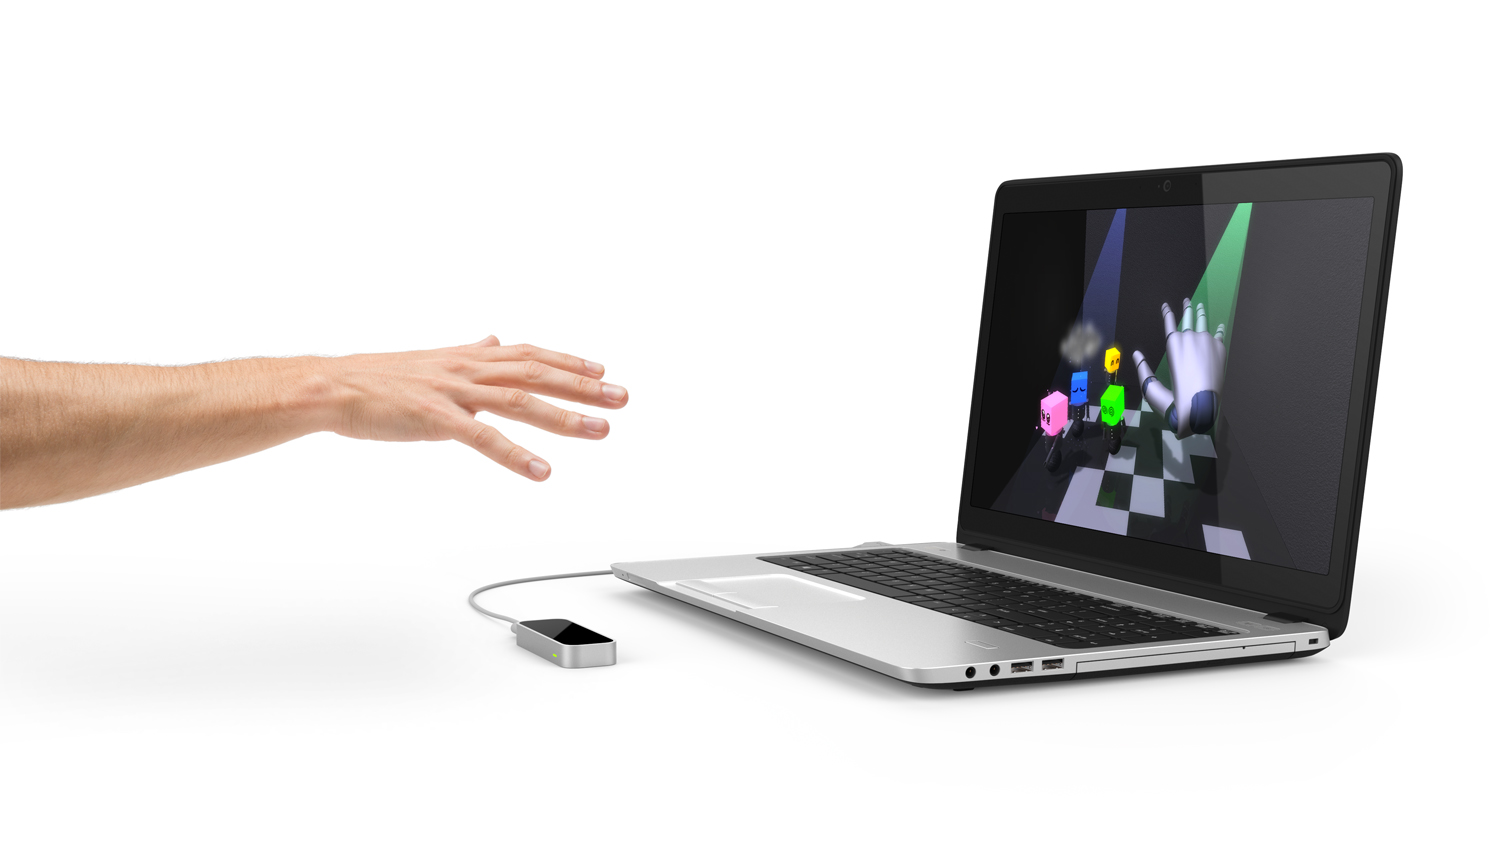
\includegraphics[width=1.0\linewidth]{images/analysis/leap_laptop.jpg}
%	\caption[Leap Motion -- Produktbild]{Leap Motion -- Produktbild \protect\cite{Leap_Motion_Motion_Controller_2015-03-27}}
%\end{wrapfigure}

Für die Erkennung der Gesten wird der Leap Motion Sensor\footcite{Leap_Motion_Motion_Controller_2015-03-27} verwendet.
Dieser erkennt Hände (inkl. einzelne Finger) und stellt Daten derer Position, Gesten und Bewegungen zur Verfügung.

\subsubsection{Technische Details}
Die Erkennung erfolgt via optische Sensoren und Infrarot Licht.
Der Leap Motion wird per USB 2.0 angeschlossen und erkennt Gesten innerhalb eines 150\textdegree-Winkels zwischen 25\,mm und 600\,mm Höhe.
Am Besten funktioniert der Sensor, wenn die Silhouette der Hand einen hohen Kontrast zur Umgebung aufweist.
Die Messdaten werden mit einem internen Handmodell kombiniert, so dass immer eine vollständige Hand als Output vorliegt.
\footcite{API_Overview__Leap_Motion_v2.2_documentation_2015-03-27}


\begin{figure}[H]
  \IfDefined{RawFloats}{\RawFloats} % required if floatrow is loaded
  \begin{minipage}[b]{0.45\linewidth}
    \centering
   	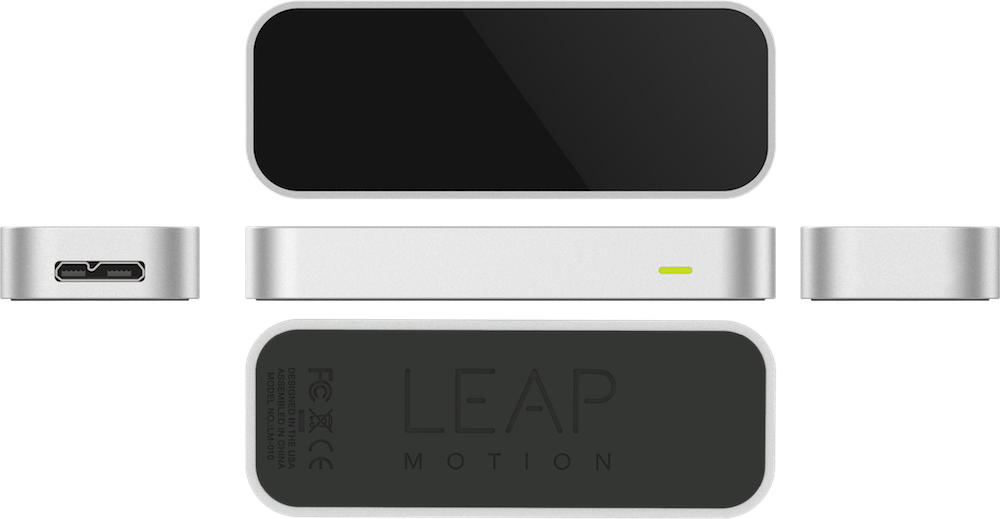
\includegraphics[width=1.0\linewidth]{images/analysis/leap_360_view.png}
   	\caption[Leap Motion von allen Seiten]{Leap Motion von allen Seiten (Quelle: \fullcite{Leap_Motion_-_VJs_Magazine_2015-03-27})}
  \end{minipage}%
  \hspace{.1\linewidth}
  \begin{minipage}[b]{0.45\linewidth}
    \centering
	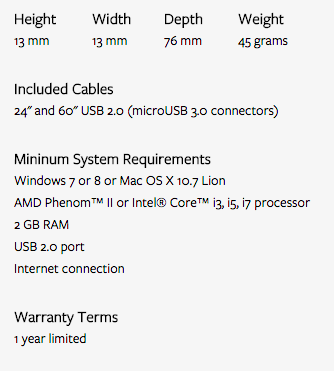
\includegraphics[width=1.0\linewidth]{images/analysis/leap_technical_specifiaction.png}
	\caption[Leap Motion - Technische Spezifikationen]{Leap Motion - Technische Spezifikationen (Quelle: \fullcite{Leap_Motion_Motion_Controller_2015-03-27})}
  \end{minipage}
\end{figure}

Weitere Informationen könne übersichtlich auf der Website des Herstellers\footcite{Leap_Motion_Motion_Controller_2015-03-27} gefunden werden.

\subsubsection{Anwendungsbereich}
\begin{wrapfigure}{R}{0.4\textwidth}
	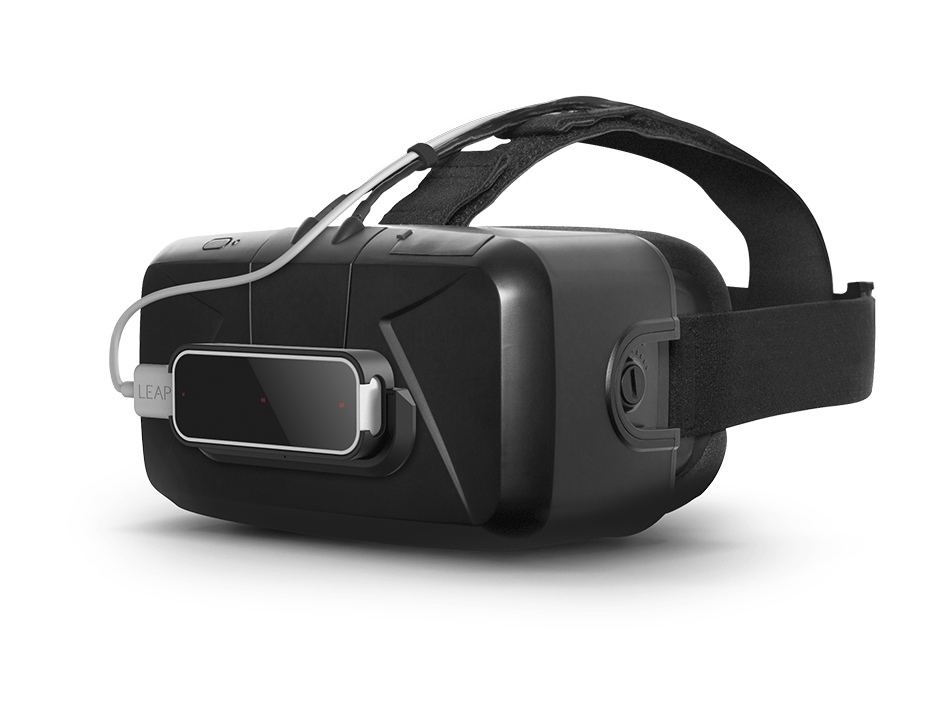
\includegraphics[width=1.0\linewidth]{images/analysis/leap_vr.png}
%	\caption[Oculus Rift VR]{\gls{vrLabel} Oculus Rift (Quelle: \fullcite{Leap_Motion_Developers_2015-03-27})}
	\caption[Oculus Rift VR]{\acrshort{vrLabel} Oculus Rift (Quelle: \fullcite{Leap_Motion_Developers_2015-03-27})}
	\label{fig:leap_vr}
\end{wrapfigure}

Der Anwendungsbereich für Gestenerkennung ist beinahe grenzenlos.
Da der Leap Motion speziell für Entwickler produziert wurde, kann der Sensor für jegliche Programme oder Steuerungen verwendet werden.

Allerdings sind Gestensteuerungen für "`gewöhnliche"' Steueraufgaben nach wie vor sehr wenig verbreitet, obwohl es theoretisch nichts intuitiveres als Gesten gibt.
Dies kann unter anderem an fehlenden Anwendungsfällen oder an falsch angesetzten Umsetzungen liegen.

Im Gesten-Entwicklungsbereich gibt es nebst den "`klassischen"' Anwendungen (wie Spiele, Scrolling, Musikkontrolle etc.) viele interessante  \gls{vrLabel}-Anwendungen. Der Sensor wird, wie in \figref{fig:leap_vr} ersichtlich ist, vorne auf einer \gls{vrLabel}-Brille befestigt und ermöglicht so eine Simulation virtueller Hände, durch welche die Steuerung erfolgt.

\subsubsection{Einrichtung}
Die Installation des Leap Motion's, gemäss der offiziellen Installationsanweisungen,\footcite{Getting_Started_Leap_Motion_Developers_2015-03-28} funktionierte auf einem OS X 10.10.2 einwandfrei.
Entsprechend sollte  die Installation auch auf einem Windows 7 oder 8 erfolgreich durchgeführt werden können.

\subsubsection{API}
\label{subsec:leapmotion:api}
% sprachen
% Aufbau der Antworten
Um den Leap Motion anzusteuern werden folgende Sprachen und Frameworks angeboten:
\begin{itemize}
	\item \textbf{JavaScript:} für Node.js oder Browser Anwendungen (siehe Beispiele\footcite{Getting_Started_Leap_Motion_Developers_2015-03-28})
	\item \textbf{Unity / C\#:} 3D Anwendungen
	\item \textbf{C++:} für hardwarenahe Anwendungen
	\item \textbf{Java}
	\item \textbf{Python}
	\item \textbf{Objective-C}: für Anwendungen auf Apple OS X
\end{itemize}

Da die Drohne ebenfalls via Python programmiert werden kann, werden alle Komponenten in Python umgesetzt und es wird nur noch auf die Python-Schnittstelle\footcite{Python_SDK_Documentation__Leap_Motion_Python_SDK_v2.2_documentation_2015-03-28} detaillierter eingegangen. Das Prinzip der verfügbaren Daten ist jedoch bei allen Schnittstellen dasselbe.

Über das \gls{apiLabel} können einzelne \glspl{glos:frameLabel} mit Infos zu erkennbaren Objekten abgerufen werden.

Folgende \textbf{Objekte} stehen pro \gls{glos:frameLabel} zur Verfügung: Hände, Finger, Knochen (Arm- und Fingerknochen) und fingerähnliche Werkzeuge (z.B. Bleistifte).
Alle Objekte werden genau identifiziert, sprich die Hände werden als rechte und linke Hand erkannt, jeder Finger als richtigen Fingertyp und jeder Fingerknochen als korrekten physikalischen Knochen. Diese Erkennung funktioniert unabhängig der Position des Objektes. Dank dem Handmodell werden nicht messbare Werte angenähert.
Jedes Objekt enthält nebst der Position einen Richtungsvektor.

Die \textbf{Veränderung} (Grösse, Drehung, Bewegung) von Objekten zwischen zwei \glspl{glos:frameLabel} kann ebenfalls abgerufen werden.

Weiter können folgende \textbf{Gesten} erkannt werden: Kneifen, Greifen, Kreisen, Wischen und Tippen.
Beim Kneifen und Greifen ist ausserdem die Stärke der Geste messbar (eins entspricht dem Maximum der möglichen Geste [z.B. einer Faust]).

\subsection{Drohne}
\label{subsec:isAnalyseDrone}
Die \textit{Crazyflie} gibt es momentan in zwei Versionen: als "`\textit{Crazyflie}"' und "`\textit{Crazyflie 2.0}"'. Verständlichkeitshalber wird im vorliegenden Dokument die erste Version "`\textit{Crazyflie}"' als "`\textit{Crazyflie 1.0}"' bezeichnet und der Begriff "`\textit{Crazyflie}"' wird für das Produkt allgemein (versionsunabhängig) verwendet.

Alle Informationen zur \textit{Crazyflie} sind im Wiki von Bitcraze vorhanden.\footcite{index_Bitcraze_Wiki_2015-03-29}

Versionsunabhängige Informationen zu  \textit{Clients}, \textit{Development}, \textit{Architcture}, \textit{\gls{apiLabel}}, \textit{Protocols} und \textit{Analysis} sind unter "`Crazyflie"' (allgemein) abgelegt.\footcite{doc_crazyflie_index_Bitcraze_Wiki_2015-03-29}

Versionsspezifische Daten der \textit{Crazyflie 2.0} werden separat aufgeführt.\footcite{projects_crazyflie2_index_Bitcraze_Wiki_2015-03-29}

\subsubsection{Technische Details}
% Protocol: http://wiki.bitcraze.se/doc:crazyflie:crtp:index
Hardwarespezifische Informationen und Überlegungen zur Architektur sind für die \textit{Crazyflie 1.0} ausführlich dokumentiert.\footcite{projects_crazyflie_hardware_explained_Bitcraze_Wiki_2015-03-29}
Während zur \textit{Crazyflie 2.0} die Angaben eher konzentriert und ergänzend zur Verfügung stehen.
\footcite{projects_crazyflie2_architecture_index_Bitcraze_Wiki_2015-03-29}
\footcite{projects_crazyflie2_hardware_specification_Bitcraze_Wiki_2015-03-29}

Die Drohne hat zwei Prozessoren. Einen für das Power- und Radiomanagement ("`nRF51822"') und eine für die eigentliche Steuerung ("`STM32F405"').

Die Kommunikation zwischen Client und Drohne erfolgt über das \gls{crtpLabel}, eigen von Bitcraze entwickelt.\footcite{doc_crazyflie_crtp_index_Bitcraze_Wiki_2015-03-30}

Folgende Werte können gemessen werden:
\begin{itemize}
	\item \textbf{"'MPU-9250"'}\footcite{MEMS_Gyro-Accel_Gyroscope_Accelerometer_Processing_-_MPU-9250_Nine-Axis_2015-03-30} (Gyro-, Accelero-, Magentometer)
	\begin{itemize}
		\item Der \textbf{Gyrometer} misst die Erdanziehungskraft auf alle drei Seiten. Damit kann die Position und die Abweichung festgestellt werden.
		\item Der \textbf{Accelerometer} misst die Beschleunigung.
		\item Der \textbf{Magentometer} misst die zwei-dimensionale Ausrichtung (Kompass) und stellt auch langsame Abweichungen, die der Gyro nicht messen kann, fest.
	\end{itemize}
	\item \textbf{"'LPS25H"'}\footcite{Class-Leading_Miniature_Pressure_Sensor_from_STMicroelectronics_Powers_New_Chapter_in_Mobile_Innovation_2015-03-30} (High precision pressure sensor)\\
	\textbf{Barometer:} Misst den Druck auf +/- 0.2\,mbar genau, damit kann die Höhe auf ca. 12\,m genau angenähert werden (was hauptsächlich auf die Abhängigkeit von Luftfeuchtigkeit und Temperatur zurückzuführen ist).
	\footcite{Barometrische_Hoehenformel__Wikipedia_2015-03-30}
\end{itemize}

\subsubsection{Entwicklung}
Anweisungen und Vorbereitungen für die Entwicklung der \textit{Crazyflie 2.0} finden sich im \textit{Getting started}.\footcite{doc_crazyflie_dev:starting_Bitcraze_Wiki_2015-03-29}

Bitcraze stellt für die Entwicklung eine vorkonfigurierte \gls{vmLabel} zur Verfügung, auf der wesentliche Programme und Repositories bereits vorhanden sind.
\footcite{projects_virtualmachine_index_Bitcraze_Wiki_2015-03-30}
So entfällt die etwas aufwändige Installation, wobei Probleme mit den USB-Geräten auftreten können. Alternativ können alle benötigten Ressourcen direkt eingerichtet werden.

Auch dabei ist das \textit{Crazyflie Client} Programm (\textit{cfclient}) für \textit{control-}, \textit{log-} und \textit{bootload-}Aufgaben.
\footcite{doc_crazyflie_client_pycfclient_index_Bitcraze_Wiki_2015-03-30}

Da bei Nutzung der \gls{vmLabel} einerseits die USB-Ports nicht korrekt durchgeleitet wurden und zudem das Key-mapping nicht "`angenehm"' eingerichtet werden konnte, wurde folgendes Setup direkt auf OS X eingerichtet:
\begin{itemize}
	\item Chip \textbf{STM32F405:} mit Firmware "`Crazyflie 2.0 2014.12.0"'\footcite{bitcraze_crazyflie-firmware_2015-03-30}
	\item Chip \textbf{nRF51822:} mit Firmware "`Version 1.1"'\footcite{bitcraze_crazyflie2-nrf-firmware_2015-03-30}
	\item \textbf{Crazyflie Client:} die Client Software "`Crazyflie PC client 2014.12.3"'\footcite{bitcraze_crazyflie-clients-python_2015-03-30}
\end{itemize}


\subsubsection{API}
\label{subsubsec:droneApi}
% doc: http://wiki.bitcraze.se/doc:crazyflie:api:python:index
% examples: https://github.com/bitcraze/crazyflie-clients-python
Die Möglichkeiten der Python API sind auf der Seite "`The Crazyflie Python API"' genau beschrieben.\footcite{doc_crazyflie_api_python_index_Bitcraze_Wiki_2015-03-30}
Einleitende Beispiele stehen auf GitHub zur Verfügung.\footcite{crazyflie-clients-python_examples_crazyflie-clients-python_2015-03-30}

In der Dokumentation wird das Flugverhalten der Drohne, abhängig den Steuerkommandos beschrieben.
Im normalen Zustand drehen die Rotoren nicht.
Sie können mit Steuerbefehle angewiesen werden.
Ein solcher Befehl ist maximal für 500\,ms, oder bis ein nächster Befehl erfolgt, gültig.
Dies schützt die Drohne bei unerwarteten Verbindungsunterbrüchen, indem die Drohne höchstens für eine halbe Sekunde unkontrolliert fliegt.
Anschliessend werden die Rotoren wieder heruntergefahren.

Um Einsteigern die Steuerung zu erleichtern, kann die Rotor-Drosselung verzögert werden, so dass die Drohne nie sprunghafte Flugmanöver ausführt.

\newpage
\subsection{Kosten}
Es folgt eine Kostenzusammenstellung der verwendeten Ressourcen:

\begin{table}[H]
	\centering
	\small\renewcommand{\arraystretch}{1.4}
	\rowcolors{1}{tablerowcolor}{tablebodycolor}
	%
	\captionabove{Kostenzusammestellung / Ausgaben}
	%
	\begin{tabularx}{0.9\textwidth}{ L{0.18\linewidth} | X | R{0.2\linewidth} }%
		Artikel & Details & Preis\\
		\hline
		\textbf{Leap Motion} & VR Developer Bundle & \euro{ 96.99 } \\
		& Shipping & \euro{ 9.99 }\\
		& \multicolumn{1}{r|}{\textit{Subtotal}} & \euro{ 106.98 }\\
		& \multicolumn{1}{r|}{\textit{Subtotal in CHF}} & CHF 132.65 \footnotemark\\
		\hline
		\textbf{Crazyflie 2.0} &  inkl. Crazyradio PA - long range 2.4 GHz USB radio dongle with antenna (110990440 - \textit{preorder}) & \textdollar{ 200.00 }\\
		& 4 x CW+CCW spare propellers (BC-CWP-01-A and BC-CCWP-01-A) (ACC01311M) & \textdollar{ 5.00 }\\
		& 1 x Spare 240mAh LiPo battery (313020007) & \textdollar{ 5.50 }\\
		& 4 x spare 7 mm motor mounts (110990444) & \textdollar{ 10.00 }\\
		& Battery holder expansion board (114990121) & \textdollar{ 4.00 }\\
		& \multicolumn{1}{r|}{\textit{Subtotal}} & \textdollar{ 224.50 }\\
		& \multicolumn{1}{r|}{\textit{Subtotal in CHF}} & CHF 222.65 \footnotemark[\value{footnote}]\\
		\hline
		\hline
		\textbf{TOTAL} & & \textbf{CHF 355.30 \footnotemark[\value{footnote}]}
	\end{tabularx}
\end{table}
\footnotetext{Die Umrechnung in CHF entspricht dem verrechneten Betrag (Kurs Ende November 2014 inkl. 1.5 \% Bearbeitungsgebühr).}



%%%

\newpage
\section{Soll-Analyse}
Die Crazyflie soll mit dem Leap Motion, via Gesten, gesteuert werden können.
Die Umsetzung soll in Python erfolgen.
% Die Lösung soll in zwei Teilen umgesetzt werden: in einer Gestenerkennung und einer Drohnensteuerung.

Die detaillierte Definition der Steuerung wird im \secref{sec:gestureControll} beschrieben.

Die Umsetzung der Steuerung (orange eingefärbt) kann in drei logische Komponenten eingeteilt werden: die Gestenerkennung, die Drohnesteuerung und die Steuerlogik.

\begin{figure}[H]
	\centering
	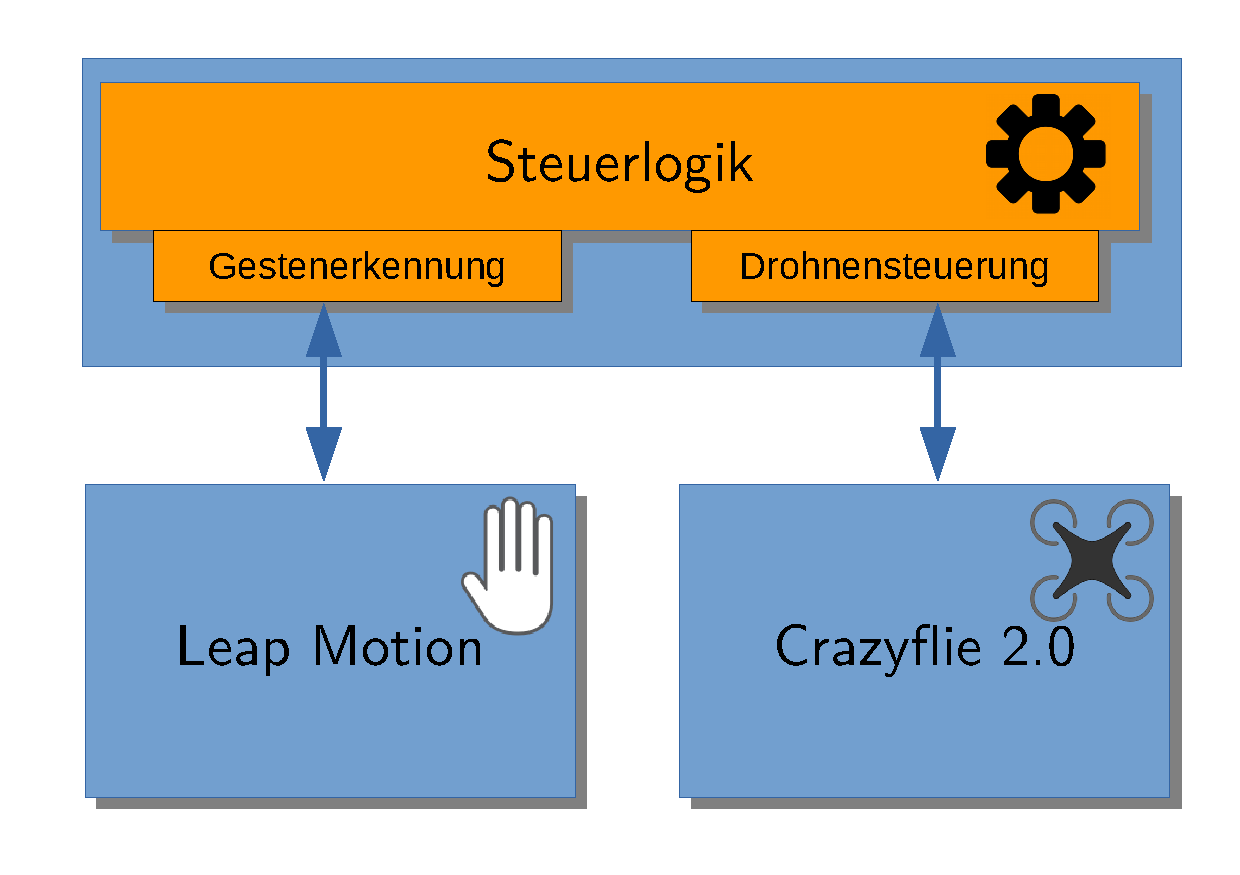
\includegraphics[width=0.8\textwidth]{figures/system_full.pdf}
	\caption{System-Überblick: Soll-Zustand}
\end{figure}

\subsection{Gestenerkennung}
Die Kompenente der Gestenerkennung, empfängt die Gesten vom Leap Motion Sensor. Die Daten werden analysiert und ausgewertet.
Eine allgemeine Gestenerkennung wird von Leap Motion zur Verfügung gestellt, die muss jedoch auf die zu erkennenden Gesten der Steuerung angepasst werden.

Die Gestenerkennung soll unabhängig der Drohne entwickelt und getestet werden können.

\subsection{Drohnesteuerung}
Die Drohne wird als alleinstehendes System betrachtet, das durch ein \gls{apiLabel} gesteuert werden kann. Zudem können Messdaten abgerufen werden. Nebst der Nutzung der \gls{apiLabel} sollten an der Drohne keine Veränderungen notwendig sein.

\subsection{Steuerlogik}
Die Steuerlogik beinhaltet das korrekte Bilden der Steuerbefehle aus den verfügbaren Gesteninformationen.
Sie verbindet die Gestenerkennung mit der Drohne.

Hier befindet sich der Hauptteil des umzusetzenden Codes. Abhängig vom Zustand der Drohne, werden andere Gesten erkannt und andere Befehle generiert.

%\subsection{Controller}
%Der Controller verbindet die Gestenerkennung mit der Drohne.
%Dazu gehören hauptsächlich zwei wiederholende Aufgaben.
%Einerseits müssen die erkannten Gesten in eine gültige Steueroperation umgeformt werden, woraus der Steuerprozess zur Drohne entsteht.
%Der Steuerprozess steuert die Drohne gemäss den Daten, die aus den Gesten gewonnen wurden, besonders für die Position wird eine aktive Steuerung benötigt, das heisst, dass die Position der Drohne auf die Zielposition der Hand angepasst werden muss. Dazu ist eine anhaltende Überprüfung und Korrektur notwendig.
